% !TEX TS-program = pdflatex
% !TEX encoding = UTF-8 Unicode

% TO COMPILE: lmake (animal scrifices may be necessary)
%%%%%%%%%%%%%%%%%%%%%%%%%%%%%%%%%%%%%%%%%%%%%%%%%%%%%%%%%%%%%%%%%%%%%%%%%%
%																							                           %
%				                         PREAMBLE      							             %
%                                                                        %
%%%%%%%%%%%%%%%%%%%%%%%%%%%%%%%%%%%%%%%%%%%%%%%%%%%%%%%%%%%%%%%%%%%%%%%%%%
\documentclass[compress]{beamer}

\mode<presentation>
{
  \usetheme{Frankfurt}
  \usecolortheme{crane}
  \setbeamercovered{transparent}
}

% Package Setup
%%%%%%%%%%%%%%%%%%%%%%%%%%%%%%%%%%%%%%%%%%%%%%%%%%%%%%%%%%%%%%%%%%%%%%%%%%
%                                                                        %
%                                 PREAMBLE                               %
%                                                                        %
%%%%%%%%%%%%%%%%%%%%%%%%%%%%%%%%%%%%%%%%%%%%%%%%%%%%%%%%%%%%%%%%%%%%%%%%%%

%% PACKAGES
\usepackage[]{lineno}
\usepackage{fancyvrb}
%\linenumbers
\usepackage{amsmath}
\usepackage{microtype}
\usepackage{algorithmic}

%% GRAPHICS RELATED
\usepackage{graphicx}
\usepackage[outdir=./tmp/]{epstopdf}
\graphicspath{{../images/}{./}{./tmp/}}
\DeclareGraphicsExtensions{.eps, .pdf, .jpeg, .png}

%% CAPTION SETUP
\usepackage{float}
\usepackage[font=footnotesize]{caption}
\usepackage[font=small]{subcaption}
\captionsetup{belowskip=12pt,aboveskip=4pt}

%% BEAMER
\usepackage{multicol}
\usepackage{multirow}
\usepackage{array}				% Table Stuff
\usepackage{arydshln}
\usepackage{rotating}

%% BIBLIOGRAPHY
\bibliographystyle{ieeetr}

%% UNITS
\usepackage{siunitx}

%% EQUATIONS
%\numberwithin{equation}{section}

%%%%%%%%%%%%%%%%%%%%%%%%%%%%%%%%%%%%%%%%%%%%%%%%%%%%%%%%%%%%%%%%%%%%%%%%%%%
%                                                                         %
%                             Listing Setup                               %
%                                                                         %
%%%%%%%%%%%%%%%%%%%%%%%%%%%%%%%%%%%%%%%%%%%%%%%%%%%%%%%%%%%%%%%%%%%%%%%%%%%
\usepackage{listings}
\lstset{ %
    language=C++,
    basicstyle=\footnotesize\ttfamily,
    numbers=left,
    numberstyle=\tiny\color{gray},
    stepnumber=2,
    numbersep=5pt,
    backgroundcolor=\color{white},
    showspaces=false,
    showstringspaces=false,
    showtabs=false,
    frame=single,
    rulecolor=\color{black},
    tabsize=2,
    breaklines=true,
    breakatwhitespace=false,
    title=\lstname,
    keywordstyle=\color{blue},
    commentstyle=\color{OliveGreen},
    stringstyle=\color{orange}
}
\DeclareCaptionFont{white}{\color{white}}
\DeclareCaptionFormat{listing}{\colorbox[cmyk]{0.43, 0.35, 0.35, 0.01}{\parbox{\dimexpr\textwidth-2\fboxsep\relax}{#1#2#3}}}
\captionsetup[lstlisting]{format=listing,labelfont=white,textfont=white,singlelinecheck=false,margin=0pt,font={bf,footnotesize}}
%\lstnewenvironment{code}[1][]%
%{ \noindent\minipage{\linewidth}
%	\lstset{#1}
%}
%{\endminipage}
%% USER COMMANDS
\usepackage{isotope}
\newcommand{\iso}{\isotope}
\newcommand{\figurewidth}{\textwidth}
\newcommand{\micron}{$\mu$m}



% Preamble / Frst Size
%\setbeamersize{text margin left=5mm, text margin right 5mm}
\title[ANS 2013] {Simulated Energy Deposition in Thin Polymeric Films}
\author[] {
    Matthew Urffer\inst{1} \and 
    A. Mabe \inst{2}  \and
    L. F. Miller \inst{1}
}
\institute[University of Tennessee] { 
  \inst{1}%
  Department of Nuclear Engineering,
  University of Tennessee, Knoxville, TN
  \\
  \inst{2}
  Department of Chemistry,
  University of Tennessee, Knoxville, TN

}

\date[] {June 19, 2013}
\pgfdeclareimage[height=0.5cm]{university-logo}{../images/utwordmarkhorz.png}
\logo{\pgfuseimage{university-logo}}

\begin{document}

\begin{frame}[plain]
  \titlepage
  \tiny
    \begin{center}
\centering{Financial support from the Domestic Nuclear Detection Office (DNDO) through Award No. 003387891 is gratefully acknowledged. 
  Any opinions, findings, and conclusions or recommendations expressed in this material are those of the presenter and do not necessarily reflect the views of DNDO.}
  \end{center}
\end{frame}

\begin{frame}{Talk Outline}
  \tableofcontents
\end{frame}


%%%%%%%%%%%%%%%%%%%%%%%%%%%%%%%%%%%%%%%%%%%%%%%%%%%%%%%%%%%%%%%%%%%%%%%%%%
%                                                                        %
%                            INTRODUCTION                                %
%                                                                        %
%%%%%%%%%%%%%%%%%%%%%%%%%%%%%%%%%%%%%%%%%%%%%%%%%%%%%%%%%%%%%%%%%%%%%%%%%%
% !TEX TS-program = pdflatex
% !TEX encoding = UTF-8 Unicode

% Matthew Urffer Master Thesis
% INTRODUCTORY MATERIAL 

\section{Introduction}

\subsection{Radiation Portal Monitors}

%%%%%%%%%%%%%%%%%%%%%%%%%%%%%%%%%%%%%%%%%%%%%%%%%%%%%%%%%%%%%%%%%%%%%%%%%%%%%%%
\begin{frame}{U.S. Border Traffic}
\begin{columns}[onlytextwidth]
\begin{column} {0.45\textwidth}
 
  \begin{itemize}
  \item Every day 932,456 people cross into the U.S. \cite{cpb_typical_2012}
    \begin{itemize}
    	\item 259,191 by air
	\item 48,073 by sea
	\item 621,874 by land
    \end{itemize}
  \item 64,483 truck, rail and sea containers \cite{cpb_typical_2012}
 \item 253,821 privately-owned vehicles \cite{cpb_typical_2012}
  \end{itemize}
\end{column}
\begin{column}{0.45\textwidth}
\centering
\begin{figure}
		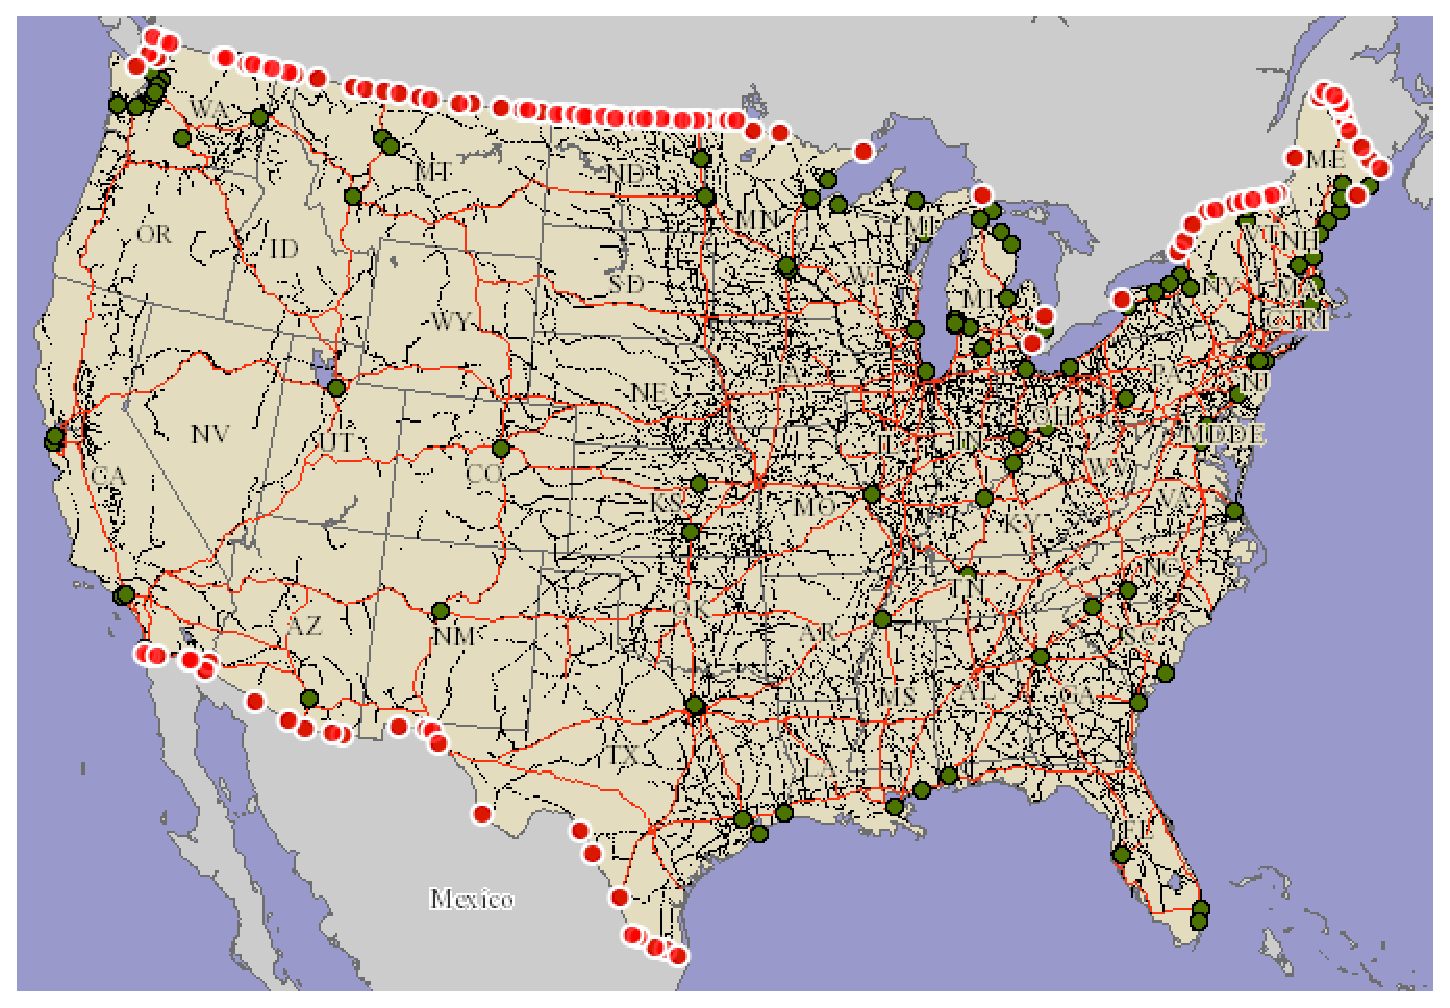
\includegraphics[width=\textwidth]{images/PortalEntryMap.eps}
		\label{fig:PortalEntryMap}
	\caption{Portal Entry Points into the U.S.}
\end{figure}
\end{column}
\end{columns}
\end{frame}

%%%%%%%%%%%%%%%%%%%%%%%%%%%%%%%%%%%%%%%%%%%%%%%%%%%%%%%%%%%%%%%%%%%%%%%%%%%%%%%
\begin{frame}{Radiation Portal Monitors}
\begin{columns}[onlytextwidth]
	\begin{column} {0.45\textwidth}
  	\begin{itemize}
  		\item Radiation portal monitors (RPMs) are passive radiation detectors
  		\item {
  			 RPMs are currently   ${}^3$He based detectors
  			\center
    		${}^3He +n \to p +{}^3H$
    	}
  		\item 
  			Shortage of ${}^3$He, so alternatives are being explored
  		\end{itemize}
	\end{column}
	\begin{column}{0.5\textwidth}
		\centering
		\begin{figure}
			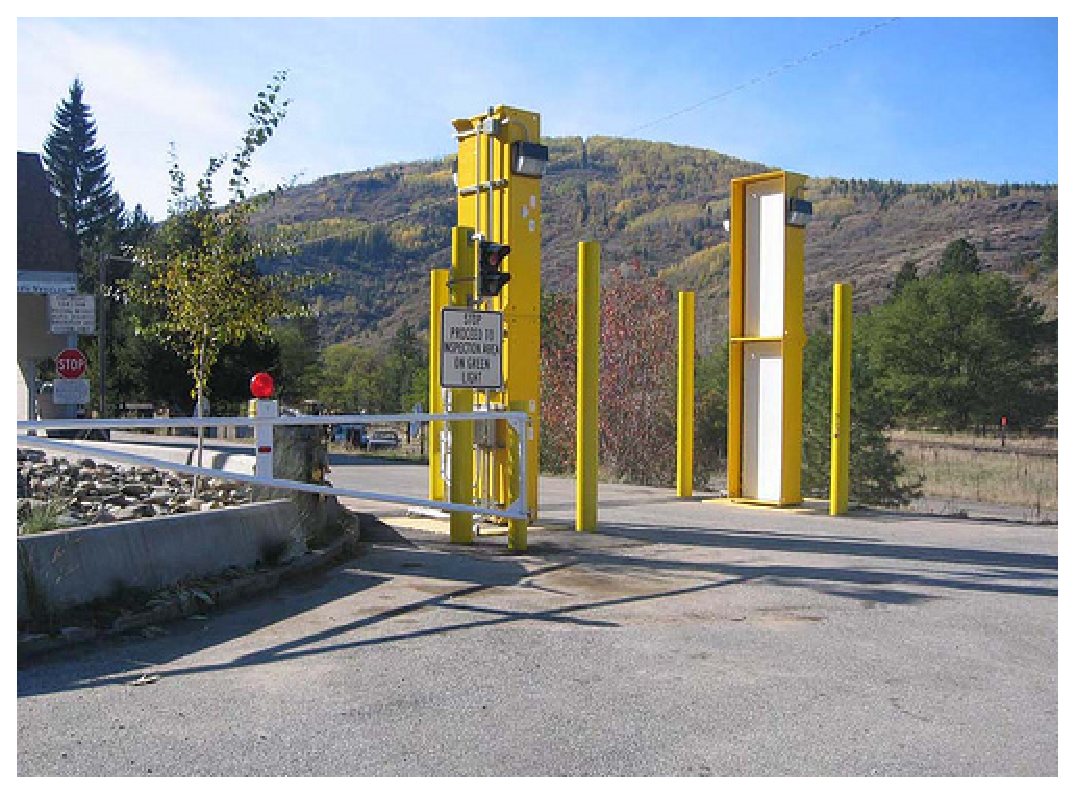
\includegraphics[width=\textwidth]{images/RPM8_Installed.eps}
			\label{fig:RPM8Installed}
			\caption{Installed RPM}
			\end{figure}
	\end{column}
\end{columns}
\end{frame}


%%%%%%%%%%%%%%%%%%%%%%%%%%%%%%%%%%%%%%%%%%%%%%%%%%%%%%%%%%%%%%%%%%%%%%%%%%%%%%%
\begin{frame}{Neutron Adsorption Interactions}
\begin{itemize}
	\item Desired reaction properties
	\begin{itemize}
		\item High probability of occurrence
		\item Ease of detecting reaction products
		\item Reaction products have a low pulse height deficit
	\end{itemize}
\end{itemize}
\begin{table}
	\tiny
	\begin{tabular}{ c | c c c} 
		Reaction                           & Q-Value (MeV) & Thermal Cross Section & Application \\
		\hline
		\hline
		${}^3He + n \to p +{}^3H$          & 0.756     & 5,330 & Proportional counter gas \\
		${}^6Li + n \to {}^3H + \alpha$    & 4.78      & 940 & Lithium glass scintillators \\
		${}^{10}B + n \to \alpha + {}^7Li$ & 2.31      & 3,840 & Plastic scintillators \\
		${}^{157}Gd + n \to \gamma$        &various    & 259,000 & various \\
	\end{tabular}
\end{table}
\end{frame}

%%%%%%%%%%%%%%%%%%%%%%%%%%%%%%%%%%%%%%%%%%%%%%%%%%%%%%%%%%%%%%%%%%%%%%%%%%%%%%%
\begin{frame}{Energy Deposition (Charged Particle)}
Products of ${}^6$Li neutron interaction are triton and alpha:
\begin{columns}[onlytextwidth]
\begin{column}{0.45\textwidth}
\begin{itemize}
	\small
	\item Alpha Energy: 2.05 MeV
	\item Triton Energy: 2.73 MeV
\end{itemize}
Alpha and tritons tend to deposit all of their energy in a small region
\end{column}
\begin{column}{0.45\textwidth}
	\begin{figure}
	\includegraphics[width=\textwidth]{images/PStarAStarRange.eps}
	\caption{Alpha and Triton Range (CSDA) \protect \cite{berger_estar_2005}}
	\label{fig:PStarAStarRange}
	\end{figure}
\end{column}
\end{columns}
\end{frame}

\subsection{Detector Requirements}
%%%%%%%%%%%%%%%%%%%%%%%%%%%%%%%%%%%%%%%%%%%%%%%%%%%%%%%%%%%%%%%%%%%%%%%%%%%%%%%
\begin{frame}{Detector Requirements}
DHS / DNDO (along with PNNL) has determined a set of objectives that replacement technologies should meet:
\begin{table}
	\tiny
	\begin{tabular}{c c }
	Parameter & Specification \\
	\hline
	\hline
	Absolute neutron detection efficiency & 2.5 cps/ng of ${}^{252}Cf$ (in specified test configuration) \\
	Intrinsic gamma-neutron detection efficiency & $ \epsilon_{int,\gamma}\leq 10^{-6}$ \\
	Gamma absolute rejection ratio for neutrons (GARRn) & $ 0.9 \leq \text{ GARRn }\leq$ 1.1 at 10 mR/h exposure \\
	Cost &  \$ 30,000 per system \\
	\hline
	\end{tabular}
\end{table}
\end{frame}

%%%%%%%%%%%%%%%%%%%%%%%%%%%%%%%%%%%%%%%%%%%%%%%%%%%%%%%%%%%%%%%%%%%%%%%%%%%%%%%
\begin{frame}{Absolute Neutron Efficiency}
\newtheorem{thm1}{Absolute Neutron Efficiency}
\begin{thm1}<1->
$$\epsilon_{abs} = \frac{\text{Counts}}{\text{Quanta Radiation Emitted}}\; \; \protect \cite{knoll_radiation_2009} $$
Constraint:
$$\epsilon_{abs} \geq 2.5\; \text{cps per ng}\; {}^{252}\text{Cf}$$
\end{thm1}
Test configuration is defined to be 1 ng ${}^{252}$Cf surrounded by 0.5 cm of lead and 2.5 cm of HDPE, with the detector midpoint 2 m from the source \cite{kouzes_alternative_2010}
\end{frame}


%%%%%%%%%%%%%%%%%%%%%%%%%%%%%%%%%%%%%%%%%%%%%%%%%%%%%%%%%%%%%%%%%%%%%%%%%%%%%%%
\begin{frame}{Intrinsic Gamma-Neutron Detection Efficiency}
\newtheorem{thm2}{Intrinsic Gamma-Neutron Detection Efficiency}
\begin{thm2}<1->
$$\epsilon_{int,n \gamma} = \frac{\text{Counts}}{\text{Quanta Radiation Crossing Detector}} \; \protect \cite{kouzes_alternative_2010} $$
Constraint:
$$ \epsilon_{int,n \gamma} \leq 10^{-6} $$
\end{thm2}
\begin{itemize}
	\item Counts over quanta crossing the detector
	\item Measured from a source that produces a 10 mR/hr field
\end{itemize}
\end{frame}

%%%%%%%%%%%%%%%%%%%%%%%%%%%%%%%%%%%%%%%%%%%%%%%%%%%%%%%%%%%%%%%%%%%%%%%%%%%%%%%
\begin{frame}{Gamma Absolute Rejection Ratio}
\newtheorem{thm3}{GARRn}
\begin{thm3}<1->
$$ GARRn = \frac{\epsilon_{\gamma,abs}}{\epsilon_{n,abs}} \; \protect \cite{kouzes_alternative_2010} $$
Constraint:
$$ 0.9 \leq GARRn \leq 1.1 $$
\end{thm3}
The detector's performance should change by no more than 10\% in a strong gamma field
\begin{itemize}
	\item GARRn is measured by exposing the detector to a 10 mR/hr gamma field while exposed to neutron source
	\item Count rate is measured when the gamma source is no longer present
	\item Difference determines the GARRn
\end{itemize}
\end{frame}

%%%%%%%%%%%%%%%%%%%%%%%%%%%%%%%%%%%%%%%%%%%%%%%%%%%%%%%%%%%%%%%%%%%%%%%%%%%%%%%
%                                                                             %
%                                PREVIOUS WORK                                %
%                                                                             %
%%%%%%%%%%%%%%%%%%%%%%%%%%%%%%%%%%%%%%%%%%%%%%%%%%%%%%%%%%%%%%%%%%%%%%%%%%%%%%%
\subsection{Previous Work}

%%%%%%%%%%%%%%%%%%%%%%%%%%%%%%%%%%%%%%%%%%%%%%%%%%%%%%%%%%%%%%%%%%%%%%%%%%%%%%%
\begin{frame}{Replacement Technologies (Boron)}
\begin{columns}[onlytextwidth]
\begin{column}{0.45\textwidth}
\begin{itemize}
	\small
	\item Boron Straw Tubes (Proportional Technology) \cite{kouzes_boron-lined_2012}
	\begin{itemize}
		\tiny
		\item Count rate meets requirements
		\item Gamma rejection is estimated to be $4x10^{-9}$
		\item GARRn within desired range
	\end{itemize}
	\small
	\item Boron Triflouride Gas Detectors (LND) \cite{kouzes_bf3_2009}
	\begin{itemize}
		\tiny
        \item Two tubes are marginally able to replace one ${}^3$He tube
		\item BF${}_3$ Tubes require 2200V to operate than ${}^3$He tubes (1000 V)
		\item BF${}_3$ Tubes require less pressure than ${}^3$He tubes
	\end{itemize}
\end{itemize}
\end{column}
\begin{column}{0.45\textwidth}
	\begin{figure}
	\centering
		\includegraphics[height=0.25\textheight]{images/B10StrawFibers.eps}
		\caption{ ${}^{10}$B Straw Fibers}
		\label{fig:B10StrawFibers}
		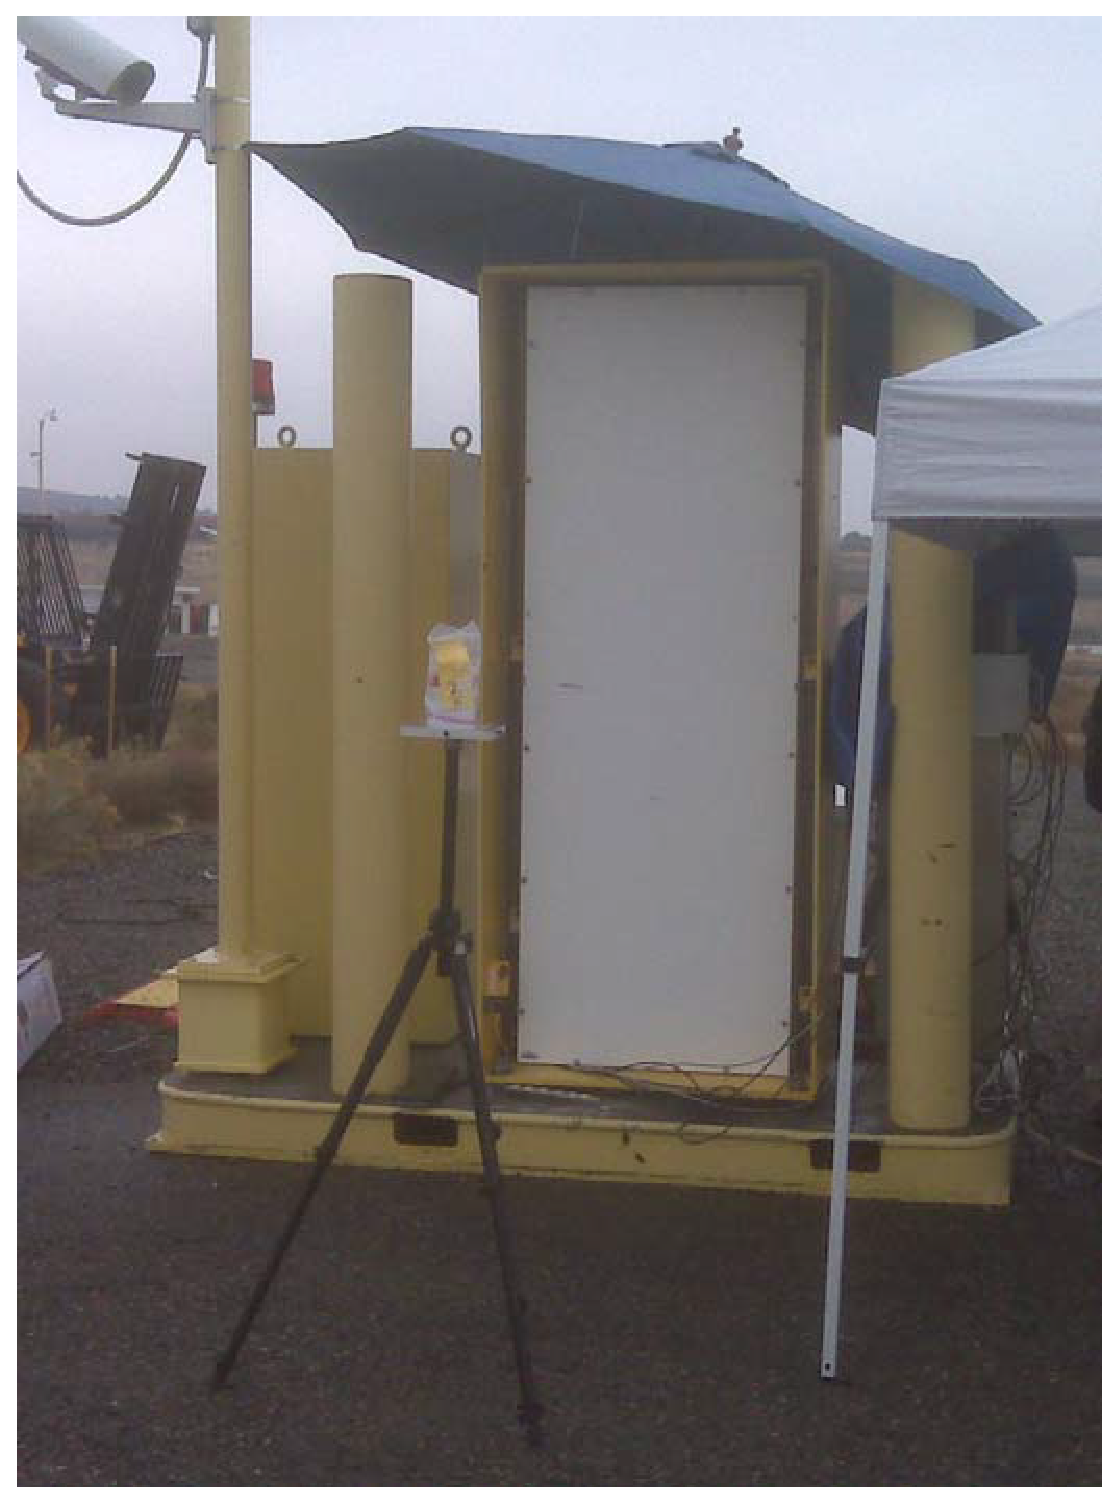
\includegraphics[height=0.25\textheight]{images/BF3Test.eps}
		\caption{PNNL test of BF${}_3$ Detector}
		\label{fig:BF3PNNLTest}
	\end{figure}
\end{column}
\end{columns}
\end{frame}

%%%%%%%%%%%%%%%%%%%%%%%%%%%%%%%%%%%%%%%%%%%%%%%%%%%%%%%%%%%%%%%%%%%%%%%%%%%%%%%
\begin{frame}{Replacement Technologies (Lithium)}
\begin{columns}[onlytextwidth]
\begin{column}{0.45\textwidth}
\begin{itemize}
	\small
	\item LiF:ZnS coated Paddles (IAT) \cite{kouzes_lithium_2010}
	\begin{itemize}
		\item Did not fulfill the neutron count rate
		\item Adequate gamma ray rejection
		\item Passed the GARRn
	\end{itemize}
	\small
	\item NucSafe Glass Fibers\cite{kouzes_alternative_2010}
	\begin{itemize}
		\item Tested with a scale model, 1.72 cps
		\item Three filter levels for GARRn
		\begin{itemize}
			\tiny
			\item Conservative filter passed GARRn, failed count rate
			\item Other filters failed GARRn
		\end{itemize}
	\end{itemize}
\end{itemize}
\end{column}
\begin{column}{0.45\textwidth}
	\begin{figure}
		\includegraphics[height=0.25\textheight]{images/LiFZnSPaddle.eps}
		\caption{${}^6$LiF:ZnS Paddle}
		\label{fig:LifZnSPaddle}
		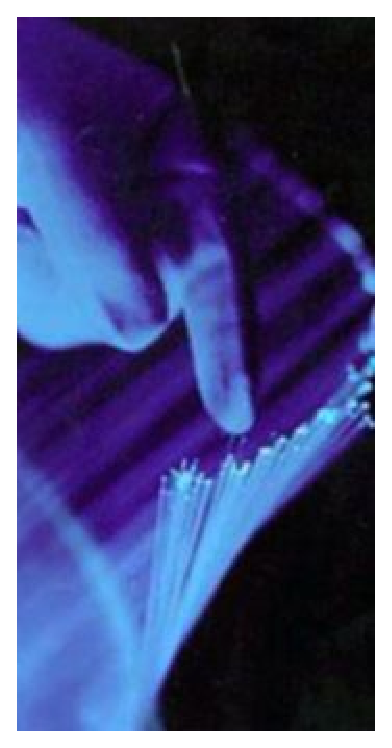
\includegraphics[height=0.25\textheight]{images/NucSafeFibers.eps}
		\caption{NucSafe Fibers}
		\label{fig:NucSafeFibers}
	\end{figure}
\end{column}
\end{columns}
\end{frame}

\section{Energy Deposition}
\subsection{Motivation}
%%%%%%%%%%%%%%%%%%%%%%%%%%%%%%%%%%%%%%%%%%%%%%%%%%%%%%%%%%%%%%%%%%%%%%%%%%
\begin{frame}{Single Collision Energy Loss}
How much energy does an electron lose in a collision?
  \newtheorem{thm1}{Single Collision Energy Loss Definition}
  \begin{thm1}<1->
    \small
    Interaction of an electron of kinetic energy E with water can be described by the probability $N(E,E')dE$ that it loses an amount of energy between $E'$ and $E'+dE$
  \end{thm1}
  \begin{itemize}
    \item $N(E,E')$ is the single collision spectrum of $E$
    \item $N(E,E')$ is a normalized probability function
  \end{itemize}
\end{frame}
%%%%%%%%%%%%%%%%%%%%%%%%%%%%%%%%%%%%%%%%%%%%%%%%%%%%%%%%%%%%%%%%%%%%%%%%%%
\begin{frame}[fragile]{Motivation}
  Secondary Electron Range Calculations:
  \begin{itemize}
    \item Low energy, high fidelity low energy electron transport needed for gamma discrimination simulation
    \item GEANT4 (with \verb+G4DNAPhysics+) provide the ability to simulate low energy electron interactions
    \item Ability to validate GEANT4 simulation
  \end{itemize}
  Neutron - Photon Discrimination:
  \begin{itemize}
    \item Secondary electrons from gamma interactions will have a higher energy than reaction products from neutron interactions
    \item Higher energies imply a partial energy deposition, thus ability for pulse height discrimination
  \end{itemize}
\end{frame}
%%%%%%%%%%%%%%%%%%%%%%%%%%%%%%%%%%%%%%%%%%%%%%%%%%%%%%%%%%%%%%%%%%%%%%%%%%
\begin{frame}{Project Goal}
  \centering
  \begin{itemize}
    \item Validate GEANT4 simulation method by reproducing single collision energy loss spectra
    \item Apply this simulation to energy deposition in films
  \end{itemize}
  \begin{figure}
    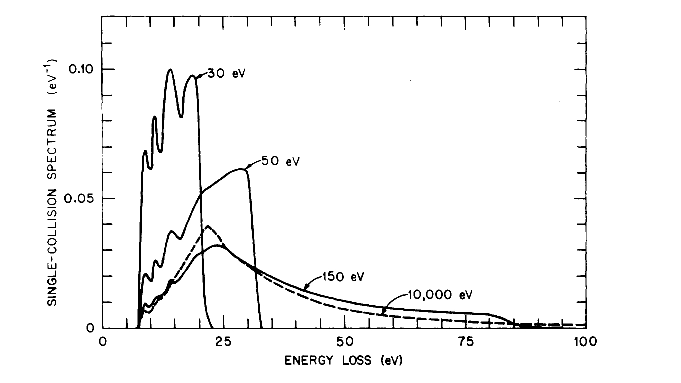
\includegraphics[width=0.6\textwidth]{Turner_Fig2_SingleCollisionELoss}
  \end{figure}
  \flushleft
  \small
  Example:
  \begin{itemize}
    \tiny
    \item For \SI{10}{\keV}, the average value of the single collision energy loss between \SI{45}{\keV} to \SI{50}{\keV} is 0.1 $\text{eV}^{-1}$
    \item Interval is \SI{5}{\keV}, so 5\% chance that a \SI{10}{\keV} electron in water has an energy loss between \SI{45}{\keV} and \SI{50}{\keV} in it's first collision
  \end{itemize}
\end{frame}
%%%%%%%%%%%%%%%%%%%%%%%%%%%%%%%%%%%%%%%%%%%%%%%%%%%%%%%%%%%%%%%%%%%%%%%%%%
\begin{frame}{Monte Carlo Simulation Modeling}
Why Monte Carlo Simulation?
\begin{itemize}
  \item Can model the physical event
  \item Analytical solutions are hard
\end{itemize}
Why GEANT4?
\begin{itemize}
  \item Develop familiarity with the toolkit
  \item GEANT4 has the ability to model low energy electrons
  \item GEANT4 has the ability to model light transport
\end{itemize}
\centering
The single collision energy loss is a simple simulation with all of the energy transfer components necessary for detailed detector energy deposition.
\end{frame}
%%%%%%%%%%%%%%%%%%%%%%%%%%%%%%%%%%%%%%%%%%%%%%%%%%%%%%%%%%%%%%%%%%%%%%%%%%
%                                                                        %
%                                METHODS                                 %
%                                                                        %
%%%%%%%%%%%%%%%%%%%%%%%%%%%%%%%%%%%%%%%%%%%%%%%%%%%%%%%%%%%%%%%%%%%%%%%%%%
\section{Methods}
\subsection{GEANT4}
\begin{frame}[fragile]{GEANT4 Introduction}
What GEANT4 is:
\begin{itemize}
  \small
  \item \href{geant4.cern.ch}{geant4.cern.ch}
  \item Free software package for the simulation of the passage of particles through matter
  \item Essentially a collection of tools for geometry, materials, physics models, events and digitization, visualizations $\dots$
  \item Maintained by the CERN community, widely used in physics
\end{itemize}
What GEANT4 is not:
\begin{itemize}
  \small
  \item For the timid
  \begin{itemize}
    \item Users are responsible for correctly implementing their own physics
    \item Users are responsible for correctly implementing their own analysis
  \end{itemize}
  \item Stagnant - major releases are still occurring
\end{itemize}
\end{frame}
%%%%%%%%%%%%%%%%%%%%%%%%%%%%%%%%%%%%%%%%%%%%%%%%%%%%%%%%%%%%%%%%%%%%%%%%%%
\begin{frame}[fragile]{GEANT4 Microdose Models}
\verb+G4DNAPhyscis+, \href{geant4-dna.in2p3.fr}{geant4-dna.in2p3.fr/index.html}
  \begin{itemize}
    \item A microdose model for modeling early biological damage by ionizing radiation on the DNA scale
    \item Electron interactions include: elastic scattering (\SI{7.4}{\eV}), electronic excitation (\SI{9}{\eV}), ionization (\SI{11}{\eV}), vibrational excitation (\SI{2}{\eV})
    \item Similar methods exist for the protons, alphas
    \item Only material defined is \verb+G4_WATER+ (NIST based)
  \end{itemize}
\end{frame}
%%%%%%%%%%%%%%%%%%%%%%%%%%%%%%%%%%%%%%%%%%%%%%%%%%%%%%%%%%%%%%%%%%%%%%%%%%
\begin{frame}[fragile]{Implemented Simulation}
  Single Collision Energy Loss:
  \begin{itemize}
     \item Electrons shot into a cube of water
     \item Initial events chosen by a particle gun
     \item Verbose tracking for first change in energy, in addition to binning on this value through ROOT
  \end{itemize}
  Energy Deposition in Thin Polymers:
  \begin{itemize}
    \item \SI{0.25}{\eV} neutrons and \iso[60]{Co} photons shot into \iso[6]{LiF} loaded polymer
    \item Energy deposition calculated for each event, binned over a run
  \end{itemize}
\end{frame}
%%%%%%%%%%%%%%%%%%%%%%%%%%%%%%%%%%%%%%%%%%%%%%%%%%%%%%%%%%%%%%%%%%%%%%%%%%
%                                                                        %
%                               RESULTS                                  %
%                                                                        %
%%%%%%%%%%%%%%%%%%%%%%%%%%%%%%%%%%%%%%%%%%%%%%%%%%%%%%%%%%%%%%%%%%%%%%%%%%
\section{Results}
\subsection{Single Collision Validation Results}
\begin{frame}{GEANT4 Single Collision Energy Loss}
  \begin{figure}
    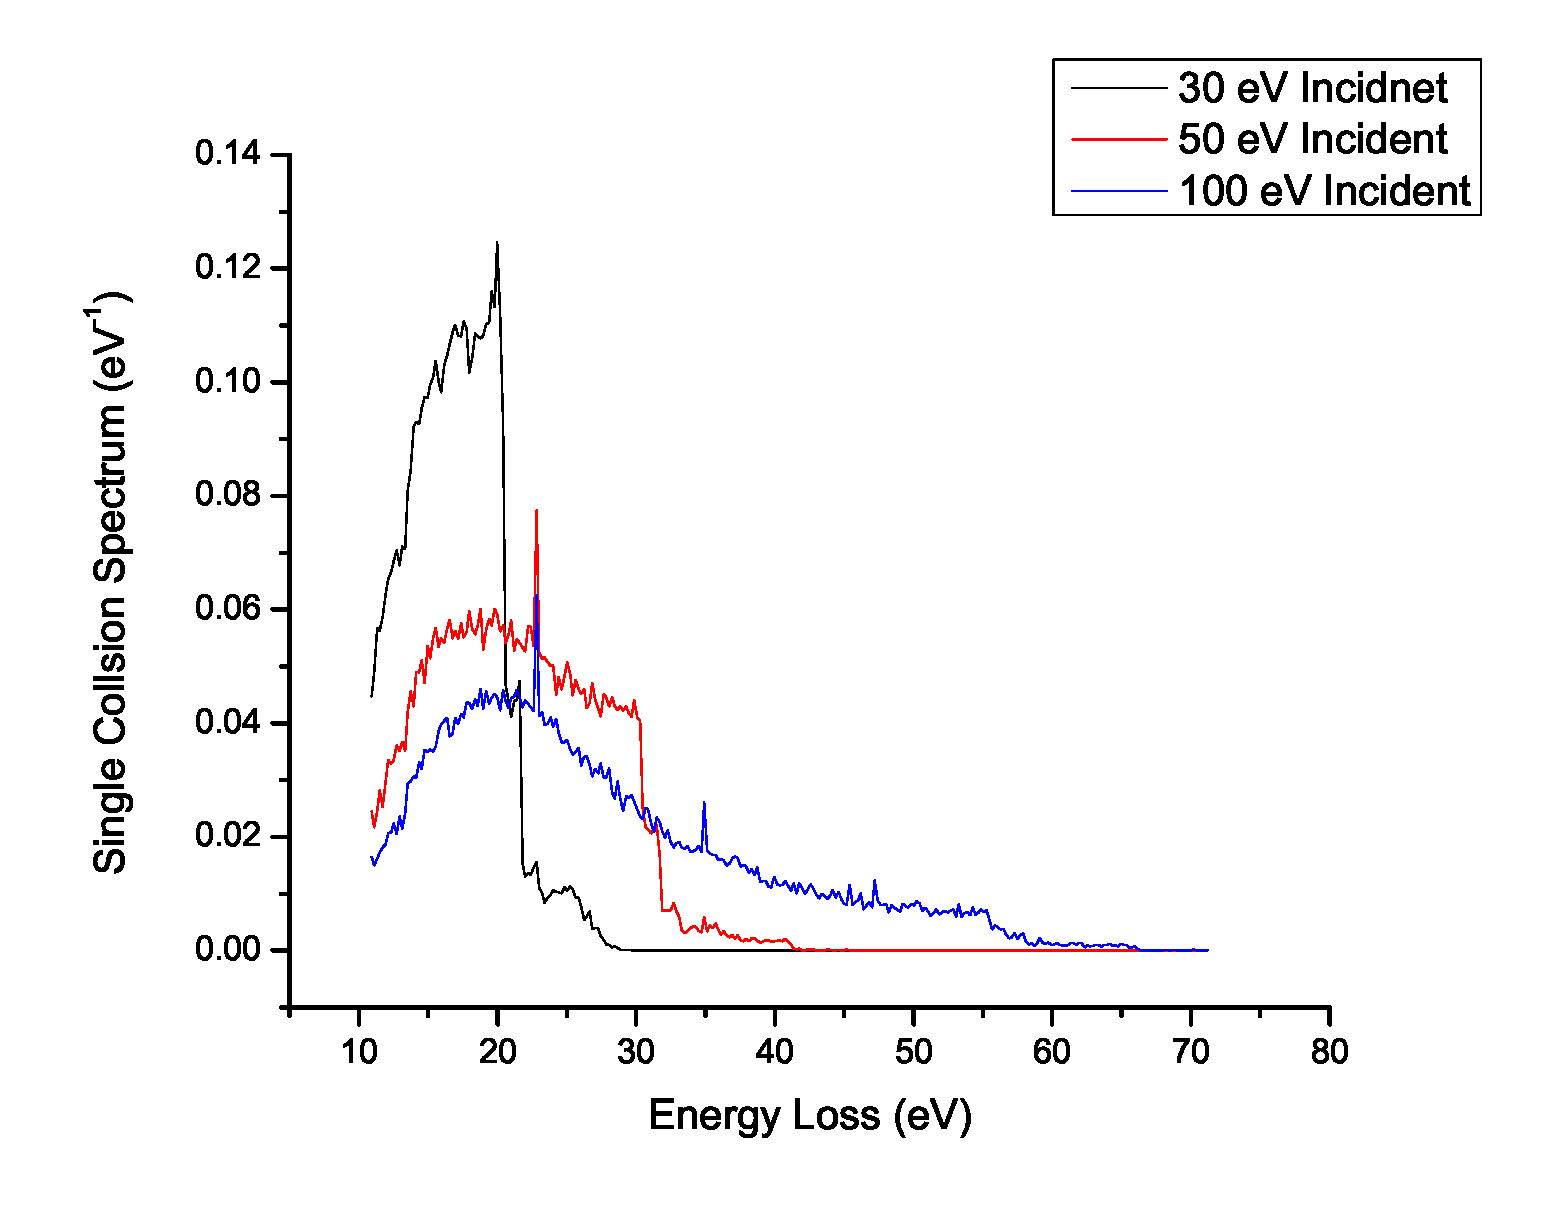
\includegraphics[width=0.75\textwidth]{SingleCollisionEnergyLoss_300bins}
  \end{figure}
\end{frame}
\begin{frame}{Comparison to Turner}
  \begin{columns}[onlytextwidth]
    \begin{column}{0.45\textwidth}
      \begin{figure}
        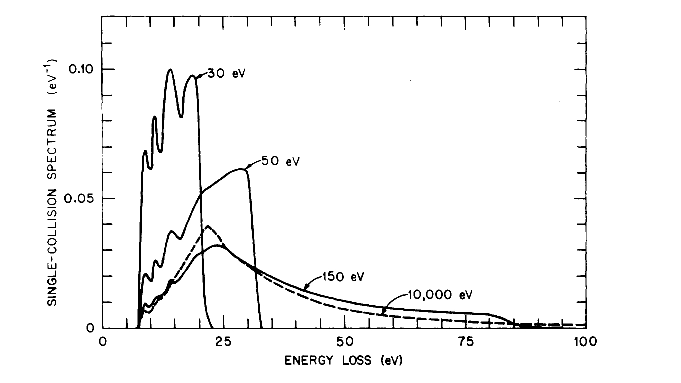
\includegraphics[width=\textwidth]{Turner_Fig2_SingleCollisionELoss}
        \caption{Tuner Spectrum}
      \end{figure}
    \end{column}
    \begin{column}{0.45\textwidth}
      \begin{figure}
        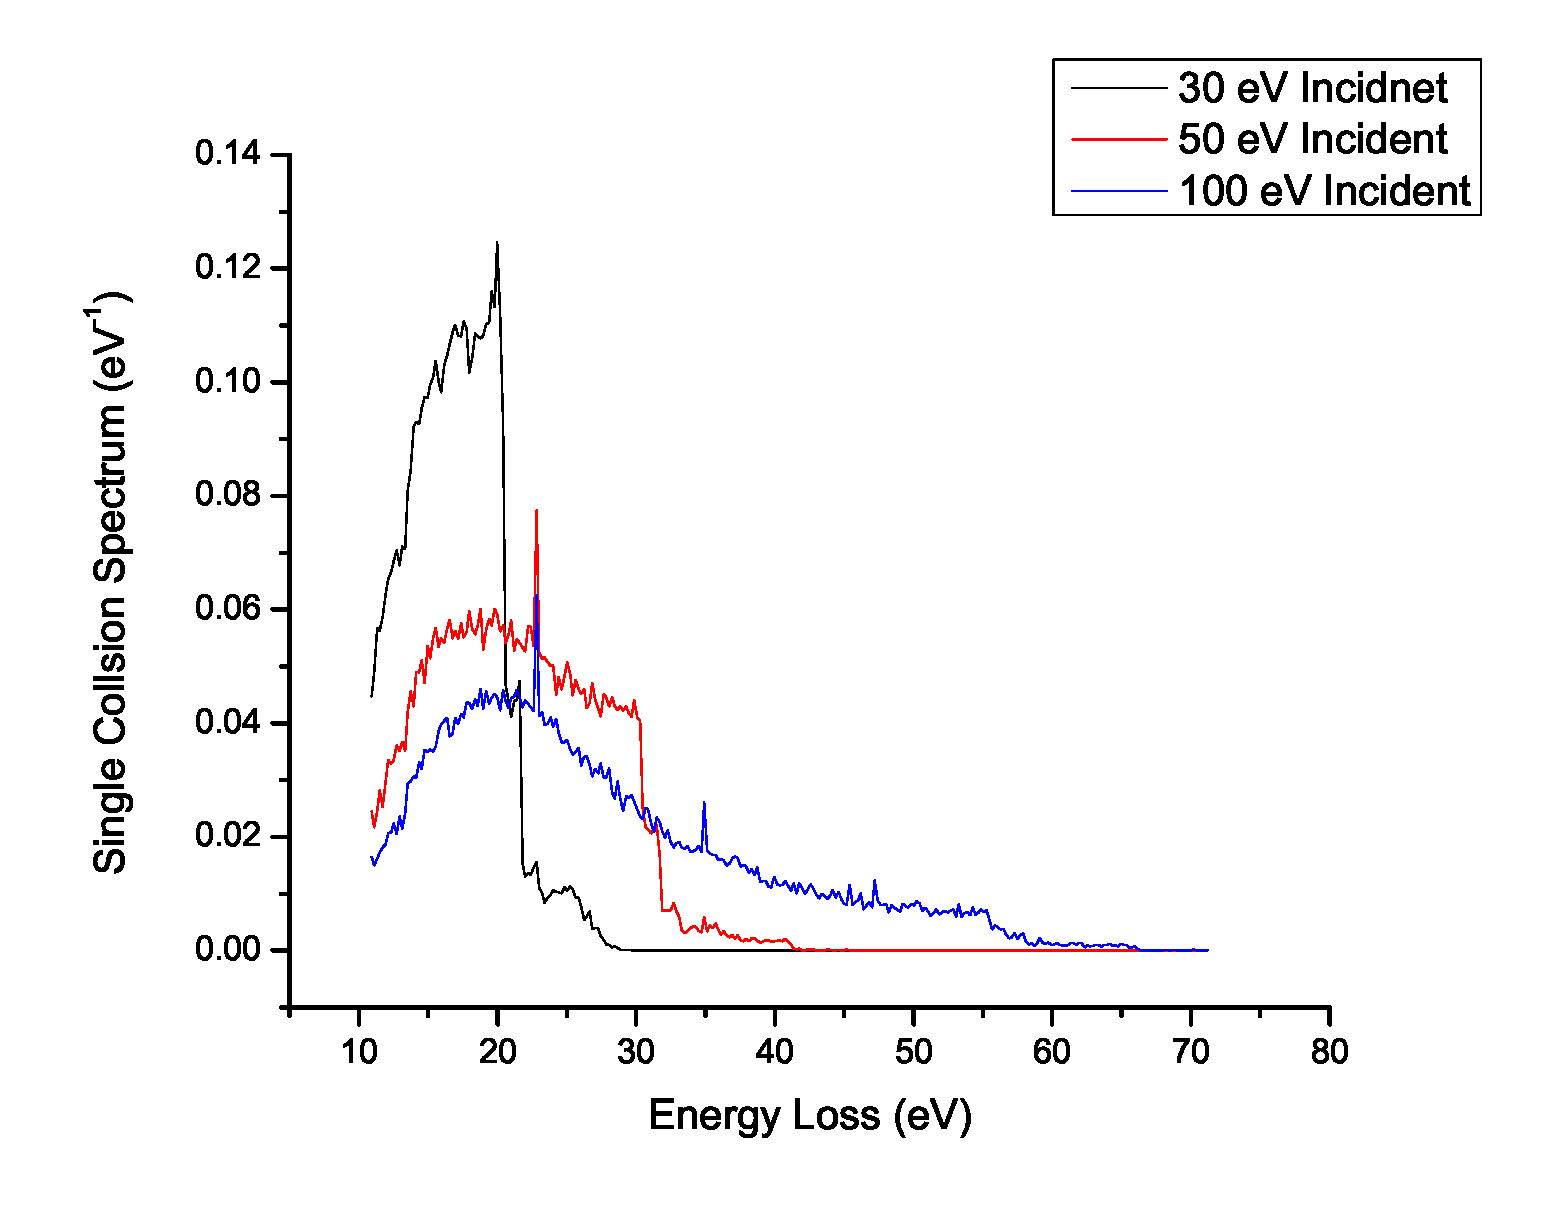
\includegraphics[width=\textwidth]{SingleCollisionEnergyLoss_300bins}
        \caption{GEANT4 Simulated Spectrum}
    \end{figure}
    \end{column}
  \end{columns}
\vspace{2mm}
Discrepancies are in the resolution of cross section data
\end{frame}
\subsection{Energy Deposition}
\begin{frame}{Comparison to Measured Spectra}
  \begin{columns}
    \begin{column}{0.45\textwidth}
      \centering
      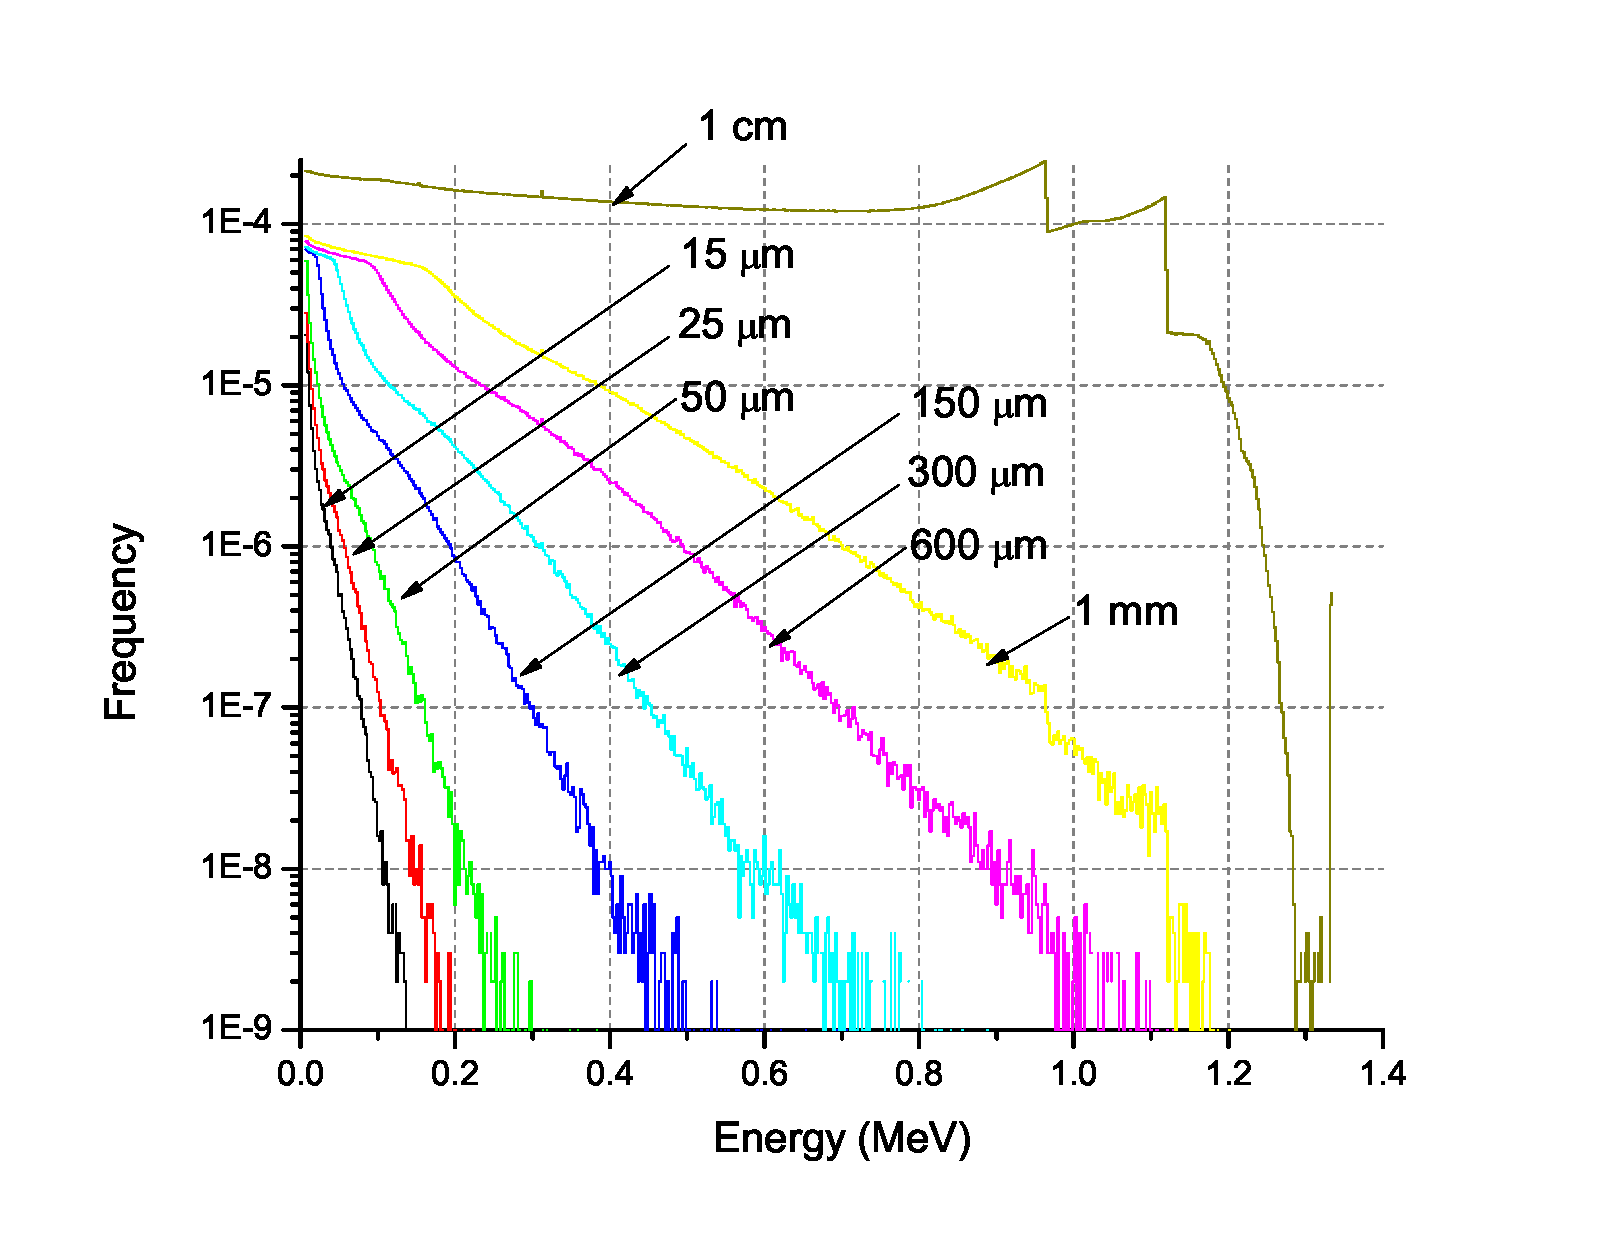
\includegraphics[width=\textwidth]{PS_EDepSim_Co60}

     GEANT4 Simulated Energy Deposition
    \end{column}
    \begin{column}{0.45\textwidth}
      \centering
      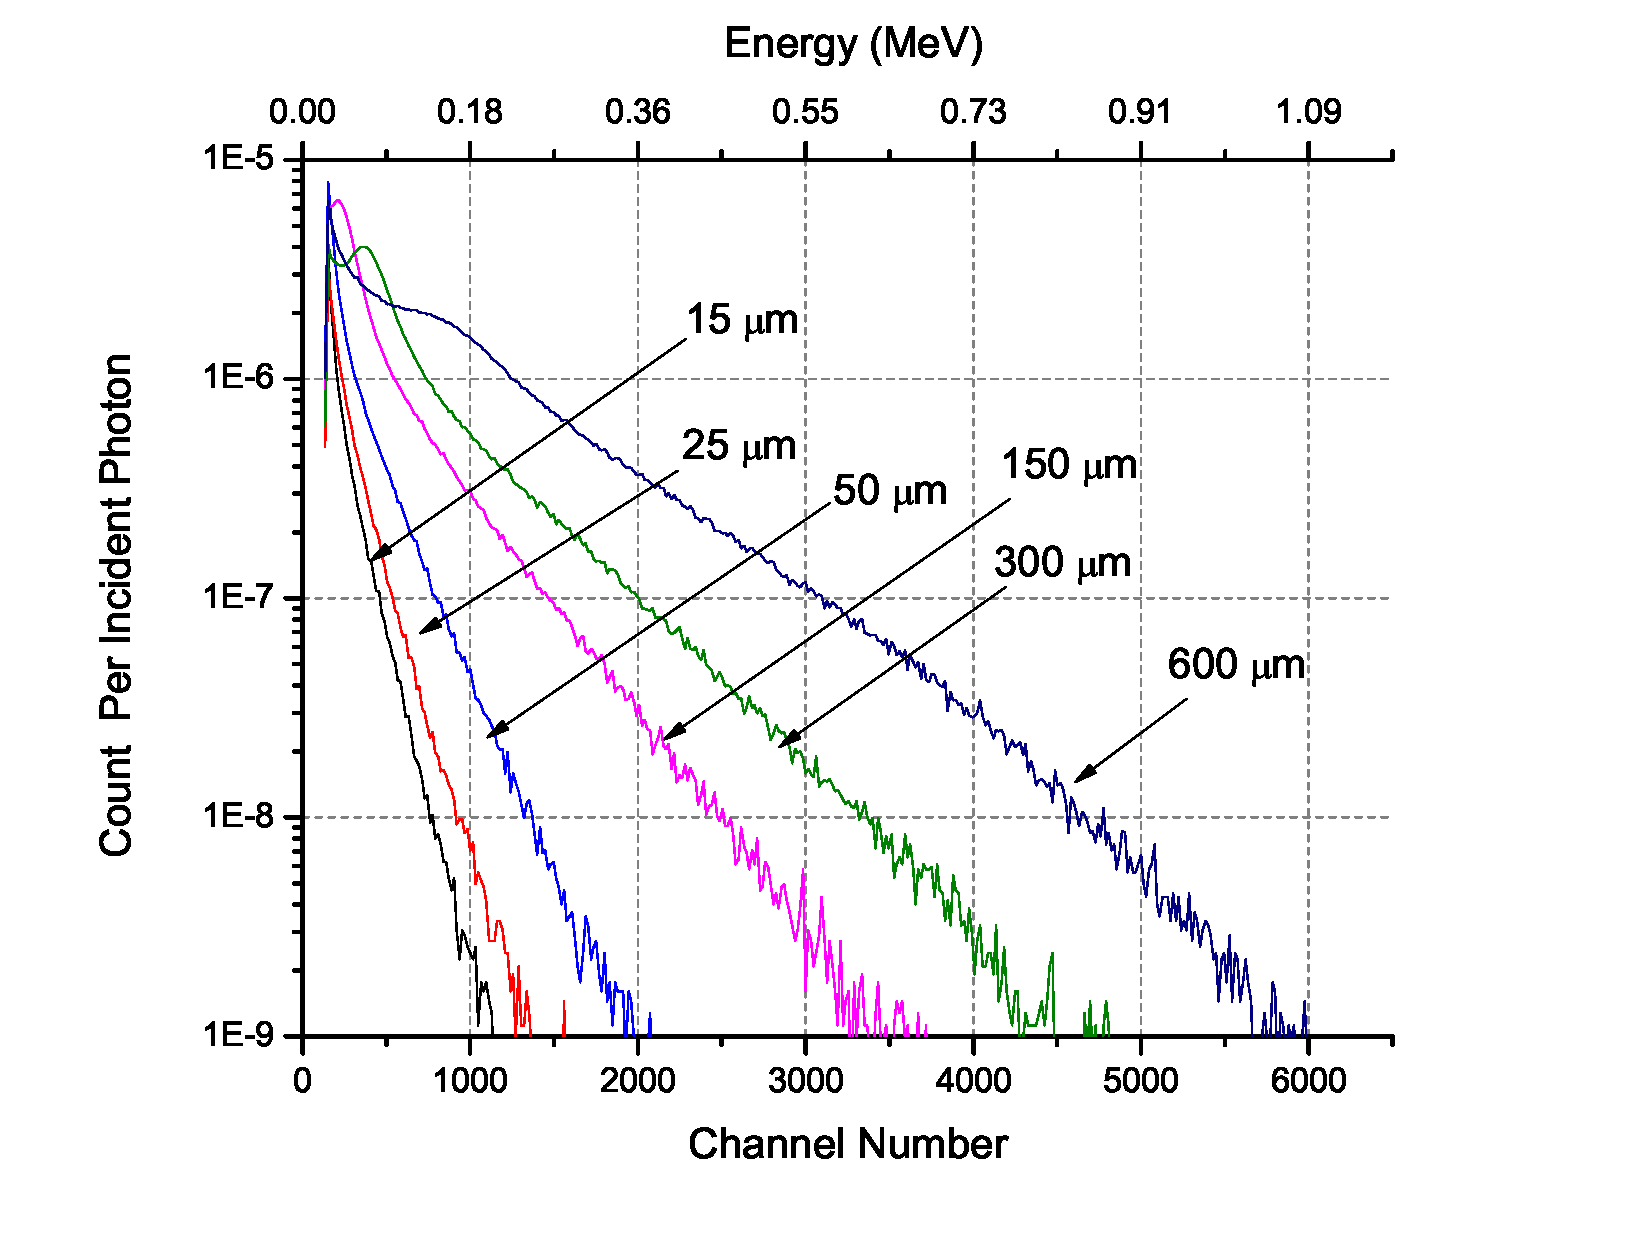
\includegraphics[width=\textwidth]{PS_GammaCR-Binned-FluxNorm_20LiF_5PPO}

      Measured Pulse Height Spectra
    \end{column}
  \end{columns}
\end{frame}
\begin{frame}{Average Light Yield and Average Energy Deposition}
  \begin{columns}
    \begin{column}{0.45\textwidth}
      \centering
      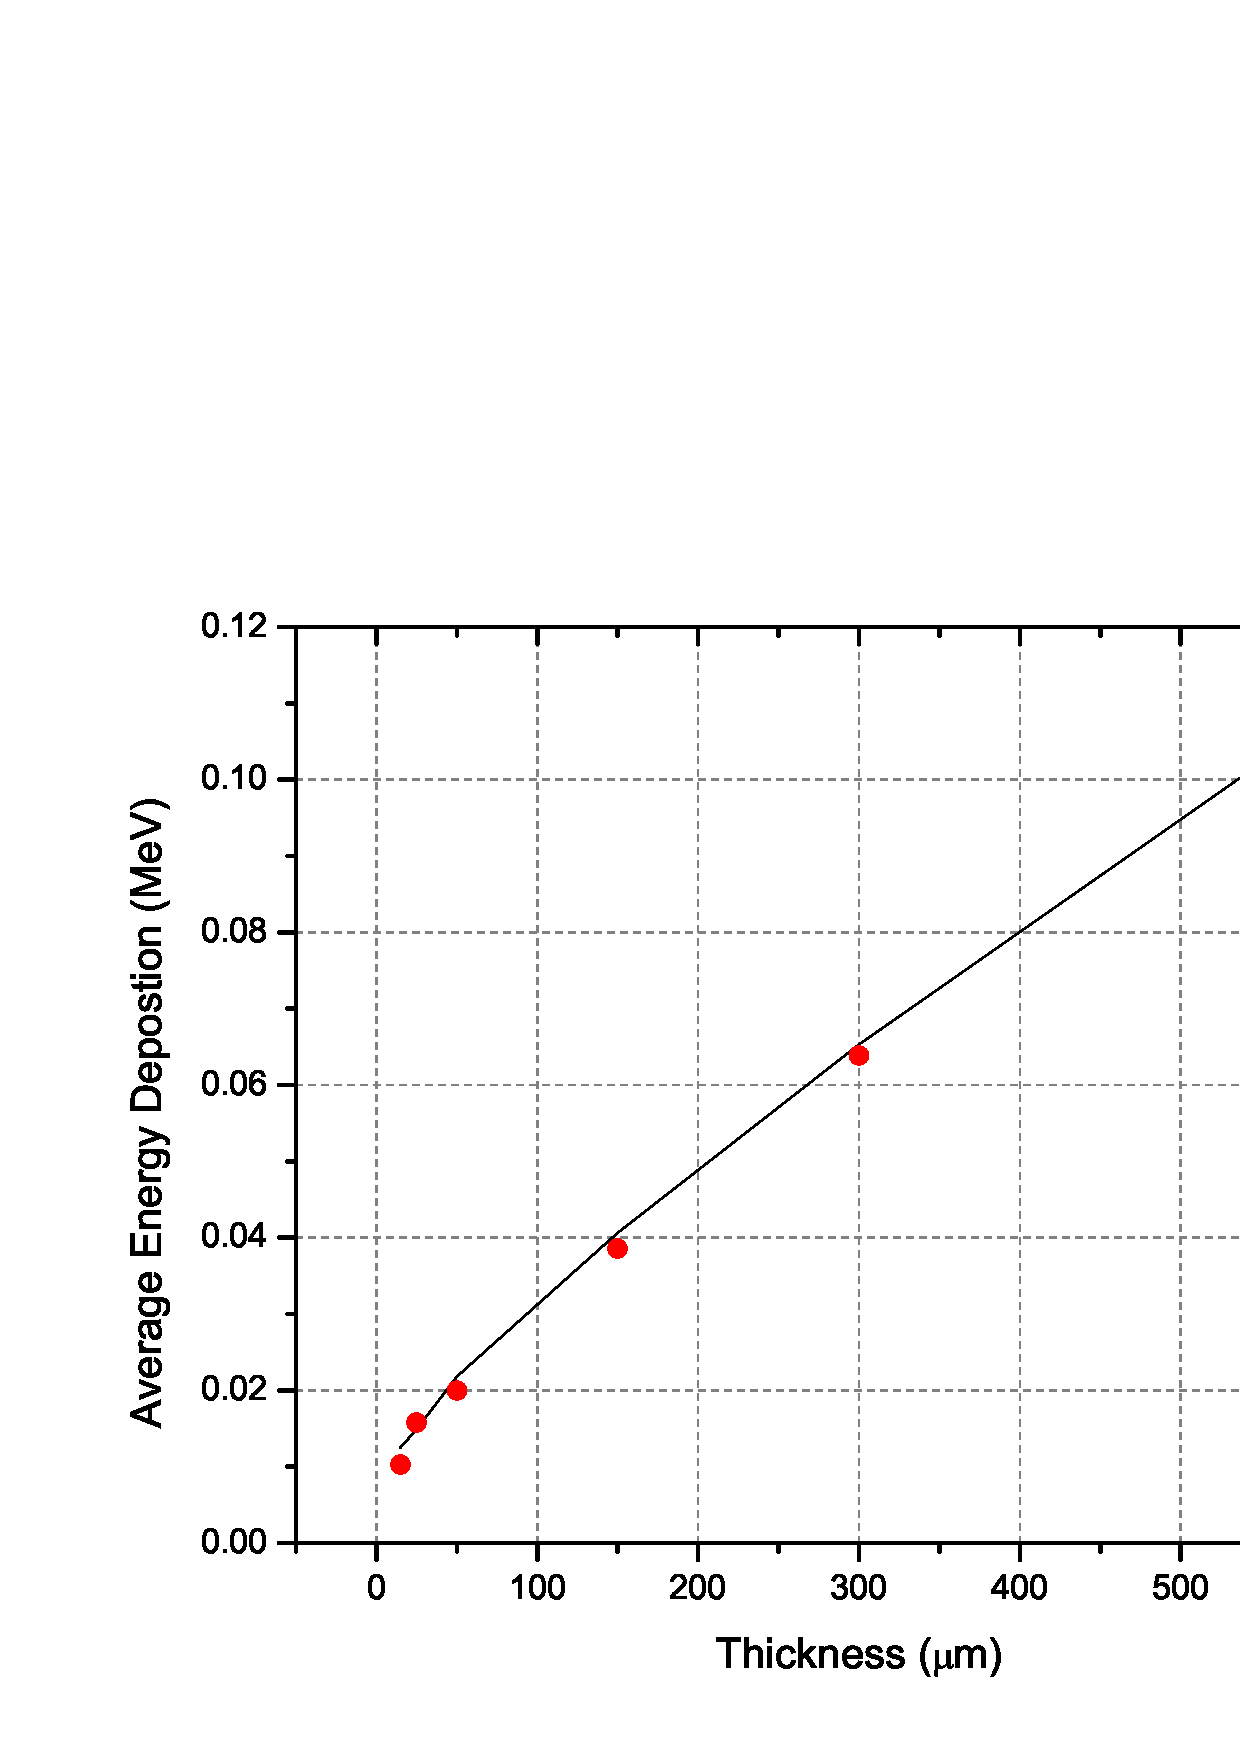
\includegraphics[width=\textwidth]{G4EDep_LightYield_Co60}

		  Gamma (\iso[60]{Co})
    \end{column}
    \begin{column}{0.45\textwidth}
      \centering
      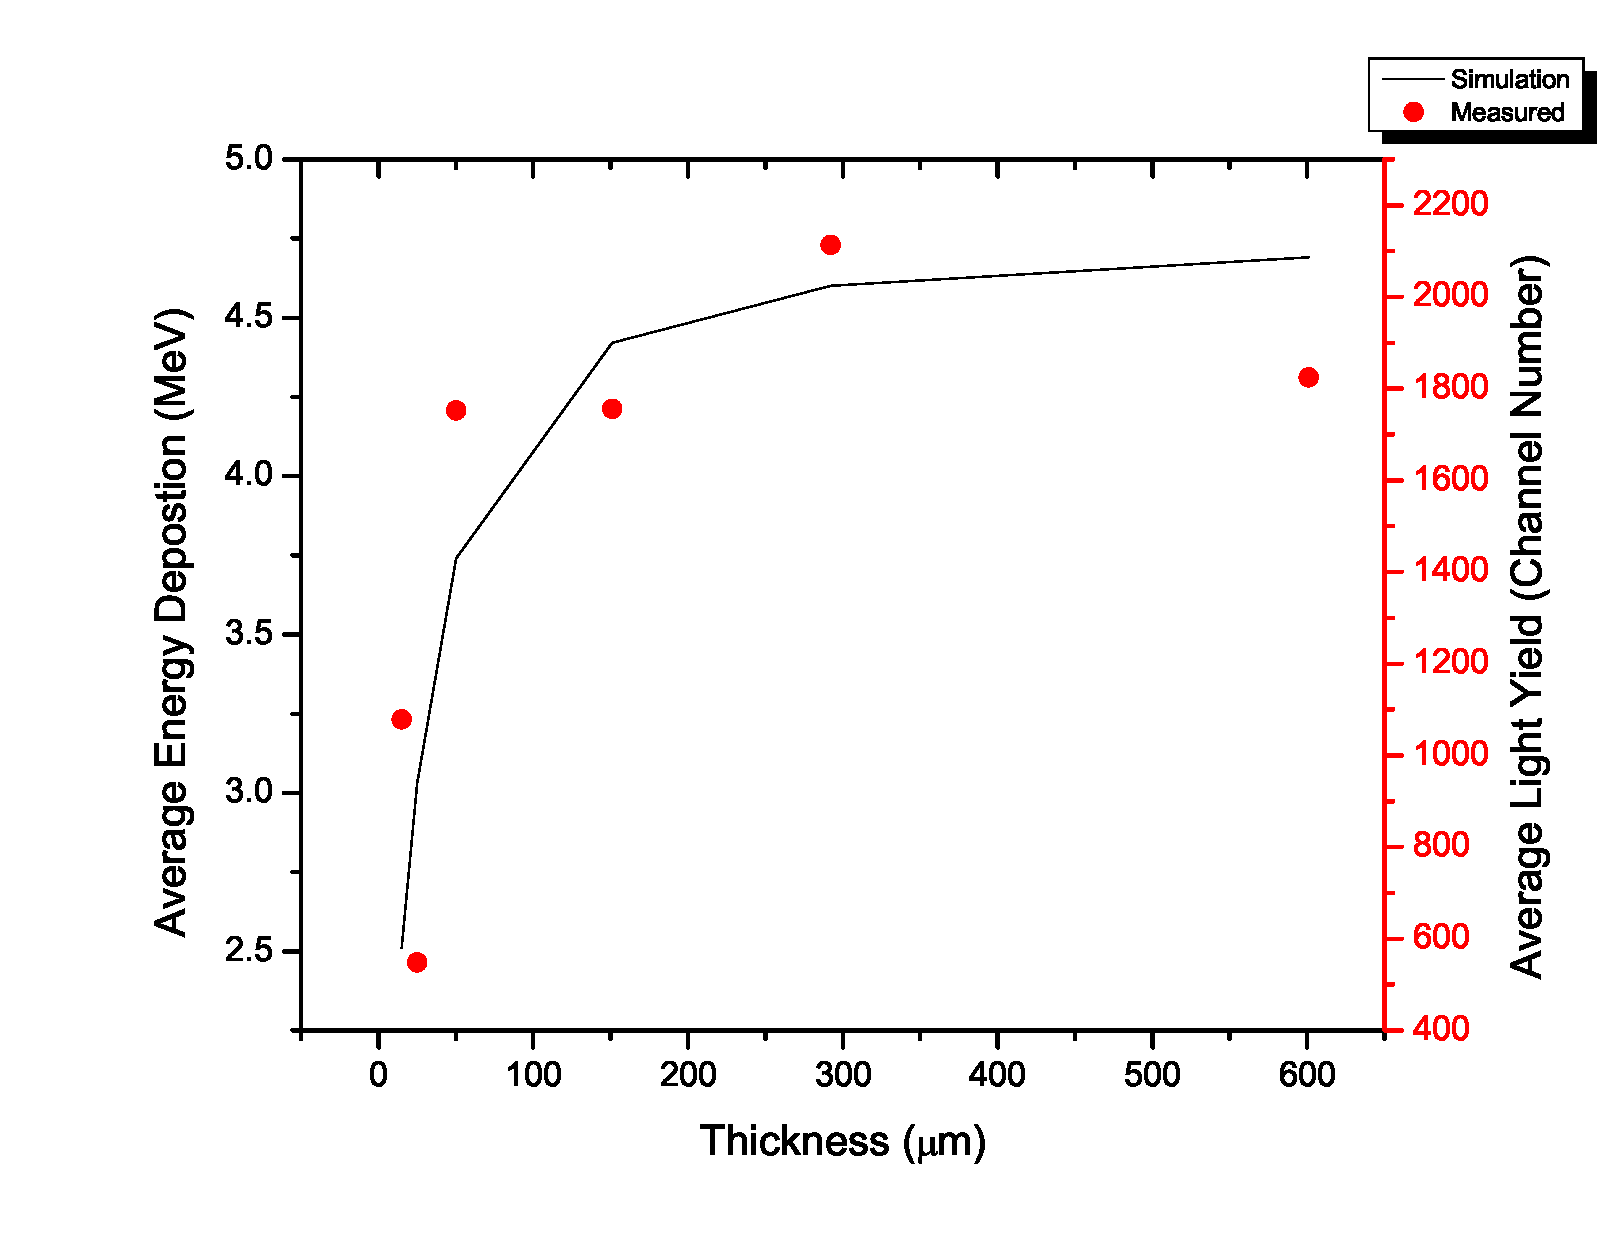
\includegraphics[width=\textwidth]{G4EDep_LightYield_Neutron}

		  Neutrons
    \end{column}
  \end{columns}
\end{frame}
%%%%%%%%%%%%%%%%%%%%%%%%%%%%%%%%%%%%%%%%%%%%%%%%%%%%%%%%%%%%%%%%%%%%%%%%%%
%                                                                        %
%                            CONCLUSIONS                                 %
%                                                                        %
%%%%%%%%%%%%%%%%%%%%%%%%%%%%%%%%%%%%%%%%%%%%%%%%%%%%%%%%%%%%%%%%%%%%%%%%%%
\section{Summary}
\begin{frame}{Summary}
  \begin{itemize}
    \item GEANT4 has the ability to accurately simulate low energy electrons in water
    \item Successfully validated a GEANT4 simulation of the energy deposition of electrons in water
    \begin{itemize}
      \item Improvements in cross sections allow for greater accuracy to be observed
      \item Same spectral shapes are observed
    \end{itemize}
  \end{itemize}
\end{frame}
\begin{frame}{Energy Deposition in thin Polymers}
  \begin{itemize}
    \item Calculated the energy deposition of \iso[60]{Co} photons and neutrons in \SI{15}{\um} to \SI{600}{\um} films
    \item Neutron - gamma discrimination can be enhanced by preferential energy deposition
  \end{itemize}
  \begin{table}[ht]
      \caption{Fractional Energy Deposition for Various Thickness}
    \centering
    \begin{tabular}{c | c c}
    Thickness & Gamma Fraction & Neutron Fraction \\
    \hline
    \hline
    \SI{15}{\um} & 0.010 & 0.531 \\
    \SI{25}{\um} & 0.013 & 0.634 \\
    \SI{50}{\um} & 0.017 & 0.782 \\
    \SI{150}{\um} & 0.032 & 0.927 \\
    \SI{300}{\um} & 0.052 & 0.964 \\
    \SI{600}{\um} & 0.087 & 0.982 \\
    \SI{1}{\mm} & 0.130 & 0.989 \\
    \SI{1}{\cm} & 0.425 & 0.998 \\
    \end{tabular}
    \label{tab:FractionEDep}
  \end{table}
\end{frame}
%%%%%%%%%%%%%%%%%%%%%%%%%%%%%%%%%%%%%%%%%%%%%%%%%%%%%%%%%%%%%%%%%%%%%%%%%%%
\begin{frame}{}
  \centering
  \begin{figure}
    
\includegraphics[height=3cm]{PowerTQuestion.png}
  \end{figure}
\end{frame}
%%%%%%%%%%%%%%%%%%%%%%%%%%%%%%%%%%%%%%%%%%%%%%%%%%%%%%%%%%%%%%%%%%%%%%%%%%%
% BILBIOLGRAPHY
\begin{frame}[plain,allowframebreaks]
\frametitle{Works Cited}
	\tiny
  \bibliography{../Zotero}
\end{frame}

\end{document}


